\documentclass[12pt,fleqn]{article}\usepackage{../common}
\begin{document}
Temel Bile�en Analizi (Principal Component Analysis -PCA-)

PCA yontemi boyut azaltan yontemlerden biridir, takip edilmeden
(unsupervised) isleyebilir. Ana fikir veri noktalarinin izdusumunun
yapilacagi yonler bulmaktir ki bu yonler baglaminda (izdusum sonrasi)
noktalarin arasindaki varyans (variance) en fazla olsun, yani noktalar
en "yaygin" sekilde bulunsunlar. Boylece birbirinden daha uzaklasan
noktalarin mesela daha rahat kumelenebilecegini umabiliriz.  Yani bir
diger amac hangi degiskenlerin varyansinin daha fazla olmasinin
gorulmesi uzerine, o degiskenlerin daha onemli olabileceginin
anlasilmasi. Ornek olarak alttaki grafige bakalim,

\begin{minted}[fontsize=\footnotesize]{python}
from pandas import *
data = read_csv("testSet.txt",sep="\t",header=None)
print data[:10]
\end{minted}

\begin{verbatim}
           0          1
0  10.235186  11.321997
1  10.122339  11.810993
2   9.190236   8.904943
3   9.306371   9.847394
4   8.330131   8.340352
5  10.152785  10.123532
6  10.408540  10.821986
7   9.003615  10.039206
8   9.534872  10.096991
9   9.498181  10.825446
\end{verbatim}

\begin{minted}[fontsize=\footnotesize]{python}
plt.scatter(data.ix[:,0],data.ix[:,1])
plt.plot(data.ix[1,0],data.ix[1,1],'rd')
plt.plot(data.ix[4,0],data.ix[4,1],'rd')
plt.savefig('pca_1.png')
\end{minted}

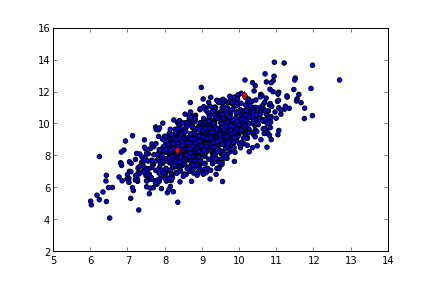
\includegraphics[height=4cm]{pca_1.png}

PCA ile yapmaya calistigimiz oyle bir yon bulmak ki, $x$ veri
noktalarinin tamaminin o yone izdusumu yapilinca sonuc olacak,
"izdusumu yapilmis" $z$'nin varyansi en buyuk olsun. Bu bir
maksimizasyon problemidir. Fakat ondan once $x$ nedir, $z$ nedir
bunlara yakindan bakalim.

Veri $x$ ile tum veri noktalari kastedilir, fakat PCA probleminde
genellikle bir "vektorun digeri uzerine" yapilan izdusumu, "daha
optimal bir $w$ yonu bulma", ve "o yone dogru izdusum yapmak"
kelimeleri kullanilir. Demek ki veri noktalarini bir vektor olarak
gormeliyiz. Eger ustte kirmizi ile isaretlenen iki noktayi alirsak (bu
noktalar verideki 1. ve 4. siradaki noktalar),

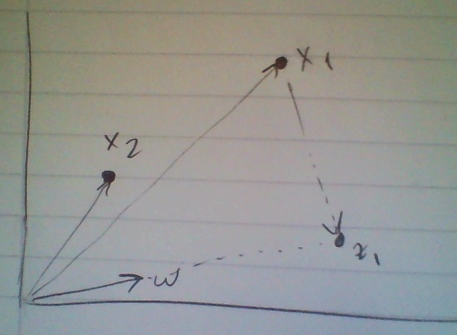
\includegraphics[height=4cm]{proj1.png}

gibi bir goruntuden bahsediyoruz. Hayali bir $w$ kullandik, ve
noktalardan biri veri noktasi, $w$ uzerine izdusum yapilarak yeni bir
vektoru / noktayi ortaya cikartiyor. Genel olarak ifade edersek, bir
nokta icin

$$z = w^T x$$

Yapmaya calistigimiz varyansi maksimize etmek demistik. Ozel bir
izdusum yonunu referans alirsak, en buyuk $Var(z_1)$'i bulacagiz. Not:
Bunu soyler soylemez $x$'i ve $z$'yi rasgele degiskenler olarak
gordugumuzu belirtmis oluyoruz. Ardi ardina alet cantasindan temsili
numaralari kullaniyoruz - $x$'i bir yandan vektor yapiyoruz, bir
yandan bir dagilimdan gelen zar atisi gibi goruyoruz, problemi
cozmemize ne yardim edecekse onu surekli devreye sokuyoruz. Devam
edelim, rasgele degisken deyince, demek ki $x,z$ dagilimlardan
gelecektir, bu dagilimlarin cok boyutlu normal (multivariate normal)
oldugunu kabul edebiliriz. Peki eger $x$, $N(\mu,\Sigma)$ gibi cok
boyutlu normal dagilimdan geliyorsa, ki $\mu$ ortalama ve $\Sigma$
kovaryanstir, $w^Tx$ nedir?

Bu yeni "seyin" beklentisi ve varyansina bakalim,

$$ E[w^Tx] = w^T E[x] = w^T \mu $$

$$ Var(w^Tx)  = w^T Var(x) w = w^T \Sigma w$$

Ustteki sonuclarin boyutlarina dikkat: $w^T \mu$ durumunda $1 \times N
\cdot N \times 1 = 1 \times 1$ , $w^T \Sigma w$ durumunda ise $1
\times N \cdot N \times N \cdot N \times 1 = 1 \times 1$.  Iki durumda
da tek boyutlu skalar degerler elde ettik. Demek ki $w^T$ ile carpim
sonrasi bir $N(w^T\mu,w^T\Sigma w)$ dagilimi elde ederiz ve bu dagilim
bir tek boyutlu bir dagilimdir. Yani $w$ yonundeki izdusum bize tek
boyutlu bir Gaussian dagilimini verecektir. Bu sonuc aslinda cok
sasirtici olmasa gerek, tum veri noktalarini alip, baslangici orijin
noktasinda olan vektorlere cevirip ayni yone isaret edecek sekilde
duzenliyoruz, bu vektorleri tekrar nokta olarak dusunursek, tabii ki
ayni yonu gosteriyorlar, bilahere ayni cizgi uzerindeki noktalara
donusuyorlar. Ayni cizgi uzerinde olmak ne demek? Tek boyuta inmis
olmak demek.

Bastaki amacimiza donersek, $Var(z_1)$'i maksimize etmek ayni anda
$Var(w_1^T\Sigma w_1)$'i maksimize etmek demektir.

Ufak bir sorun $w_1^T\Sigma w_1$'i surekli daha buyuk $w_1$'lerle
sonsuz kadar buyutebilirsiniz. Bize ek bir kisitlama sarti daha lazim,
bu sart $||w|| = 1$ olabilir, yani $w$'nin norm'u 1'den daha buyuk
olmasin. Boylece optimizasyon $w$'nin buyuklugu uzerinde taklalar
atmayacak, sadece yon bulmak ile ilgilenecek, iyi, zaten biz $w$'nin
yonu ile ilgileniyoruz. Aradigimiz ifadeyi yazalim, ve ek siniri
Lagrange ifadesi olarak ekleyelim, ve yeni bir $L$ ortaya cikartalim,

$$ L(w_1,\lambda) =  w_1^T \Sigma w_1  - \lambda(w_1^T w_1 - 1) $$

Niye eksiden sonraki terim o sekilde eklendi? O terim oyle sekilde
secildi ki, $\partial L / \partial \lambda = 0$ alininca $w_1^Tw_1 =
1$ geri gelsin / ortaya ciksin [2, sf 340], bu Lagrange'in dahice
bulusu. Bunu kontrol edebilirsiniz, $\lambda$ 'ya gore turev alirken
$w_1$ sabit olarak yokolur, parantez icindeki ifadeler kalir ve sifira
esitlenince orijinal kisitlama ifadesi geri gelir. Simdi

$$ \max\limits_{w_1} L(w_1,\lambda) $$

Turevi $w_1$'e gore alirsak, ve sifira esitlersek,

$$ 2w_1 \Sigma - 2 \lambda w_1 = 0 $$

$$ 2w_1 \Sigma = 2 \lambda w_1 $$

$$ \Sigma w_1  = \lambda w_1 $$

Ustteki ifade ozdeger, ozvektor ana formulune benzemiyor mu?
Evet. Eger $w_1$, $\Sigma$'nin ozvektoru ise ve esitligin sagindaki
$\lambda$ ona tekabul eden ozdeger ise, bu esitlik dogru olacaktir.

Peki hangi ozdeger / ozvektor maksimal degeri verir? Unutmayalim,
maksimize etmeye calistigimiz sey $w_1^T \Sigma w_1$ idi

Eger $\Sigma w_1  = \lambda w_1$ yerine koyarsak

$$ w_1^T \lambda w_1 =  \lambda w_1^T  w_1 = \lambda $$

Cunku $w_1^T w$'nin 1 olacagi sartini koymustuk. Neyse, maksimize
etmeye calistigimiz deger $\lambda$ cikti, o zaman en buyuk $\lambda$
kullanirsak, en maksimal varyansi elde ederiz, bu da en buyuk
ozdegerin ta kendisidir.

Demek ki izdusum yapilacak "yon" kovaryans $\Sigma$'nin en buyuk
ozdegerine tekabul eden ozvektor olarak secilirse, temel bilesenlerden
en onemlisini hemen bulmus olacagiz.

Cebirin geri kalani $w_2$,$w_3$ icin devam eder, bu turetmenin
detaylarini [1] ve [2] gibi kaynaklarda bulabilirsiniz. Fakat ulasilan
sonuc en bilesenlerin onem sirasinin aynen ozdegerlerin buyukluk
sirasina tekabul ediyor olmasi.

Ornek

Simdi tum bunlari bir ornek uzerinde gorelim. Iki boyutlu ornek veriyi
ustte yuklemistik. Simdi veriyi "sifirda ortalayacagiz" yani her kolon
icin o kolonun ortalama degerini tum kolondan cikartacagiz. PCA ile
islem yaparken tum degerlerin sifir merkezli olmasi gerekiyor.

Daha sonra ozdegerlerini, vektorlerini hesaplayabilmek icin verinin
kovaryansini hesaplayacagiz.

\begin{minted}[fontsize=\footnotesize]{python}
import numpy.linalg as lin
from pandas import *
data = read_csv("testSet.txt",sep="\t",header=None)
print data[:10]

means = data.mean()
meanless_data = data - means
cov_mat = np.cov(meanless_data, rowvar=0)
eigs,eigv = lin.eig(cov_mat)
eig_ind = np.argsort(eigs)
print eig_ind
\end{minted}

\begin{verbatim}
           0          1
0  10.235186  11.321997
1  10.122339  11.810993
2   9.190236   8.904943
3   9.306371   9.847394
4   8.330131   8.340352
5  10.152785  10.123532
6  10.408540  10.821986
7   9.003615  10.039206
8   9.534872  10.096991
9   9.498181  10.825446
[0 1]
\end{verbatim}

\begin{minted}[fontsize=\footnotesize]{python}
print eigs[1],eigv[:,1].T
print eigs[0],eigv[:,0].T
\end{minted}

\begin{verbatim}
2.89713495618 [-0.52045195 -0.85389096]
0.366513708669 [-0.85389096  0.52045195]
\end{verbatim}

En buyuk olan yonu quiver komutunu kullanarak orijinal veri seti
uzerinde gosterelim,

\begin{minted}[fontsize=\footnotesize]{python}
plt.scatter(data.ix[:,0],data.ix[:,1]) 
# merkez 9,9, tahminen secildi
plt.quiver(9,9,eigv[1,1],eigv[0,1],scale=10,color='r') 
plt.savefig('pca_2.png')
\end{minted}

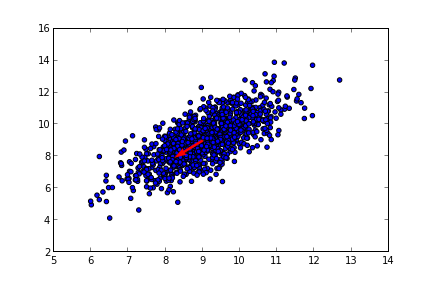
\includegraphics[height=4cm]{pca_2.png}

Goruldugu gibi bu yon hakikaten dagilimin, veri noktalarinin en cok
yayilmis oldugu yon. Demek ki PCA yontemi dogru sonucu buldu. Her iki
yonu de cizersek,

\begin{minted}[fontsize=\footnotesize]{python}
plt.scatter(data.ix[:,0],data.ix[:,1]) 
plt.quiver(9,9,eigv[1,0],eigv[0,0],scale=10,color='r') 
plt.quiver(9,9,eigv[1,1],eigv[0,1],scale=10,color='r')
plt.savefig('pca_3.png')
\end{minted}

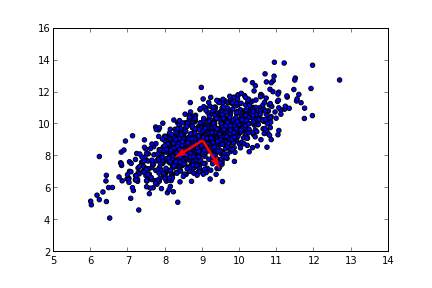
\includegraphics[height=4cm]{pca_3.png}

Bu ikinci yon birinciye dik olmaliydi, ve o da bulundu. Aslinda iki
boyut olunca baska secenek kalmiyor, 1. yon sonrasi ikincisi baska bir
sey olamazdi, fakat cok daha yuksek boyutlarda en cok yayilimin oldugu
ikinci yon de dogru sekilde geri getirilecekti.

SVD ile PCA Hesaplamak

PCA bolumunde anlatilan yontem temel bilesenlerin hesabinda ozdegerler
ve ozvektorler kullandi. Alternatif bir yontem Tekil Deger Ayristirma
(Singular Value Decomposition -SVD-) uzerinden bu hesabi
yapmaktir. SVD icin Lineer Cebir Ders 29'a bakabilirsiniz. Peki
ne zaman klasik PCA ne zaman SVD uzerinden PCA kullanmali? Bir cevap
belki mevcut kutuphanelerde SVD kodlamasinin daha iyi olmasi,
ayristirmanin ozvektor / deger hesabindan daha hizli isleyebilmesi [6].

Ayrica birazdan gorecegimiz gibi SVD, kovaryans matrisi uzerinde
degil, $A$'nin kendisi uzerinde isletilir, bu hem kovaryans hesaplama
asamasini atlamamizi, hem de kovaryans hesabi sirasinda ortaya
cikabilecek numerik puruzlerden korunmamizi saglar (cok ufak
degerlerin kovaryans hesabini bozabilecegi literaturde
bahsedilmektedir).

PCA ve SVD baglantisina gelelim:

Biliyoruz ki SVD bir matrisi su sekilde ayristirir

$$A = USV^T$$

$U$ matrisi $n \times n$ dikgen (orthogonal), $V$ ise $m \times m$
dikgen. $S$'in sadece kosegeni uzerinde degerler var ve bu  $\sigma_j$
degerleri $A$'nin tekil degerleri (singular values) olarak biliniyor.

Simdi $A$ yerine $AA^T$ koyalim, yani $A$'nin kovaryans matrisinin SVD
ayristirmasini yapalim, acaba elimize ne gececek?

$$ AA^T = (USV^T)(USV^T)^T $$

$$ = (USV^T)(V S^T U^T) $$

$$ = U S S^T U^T $$

$S$ bir kosegen matrisi, o zaman $SS^T$ matrisi de kosegen, tek farkla
kosegen uzerinde artik $\sigma_j^2$ degerleri var. Bu normal.

$SS^T$ yerine $\Lambda$ sembolunu kullanalim, ve denklemi iki taraftan
(ve sagdan) $U$ ile carparsak (unutmayalim $U$ ortanormal bir matris
ve $U^T U = I$),

$$ AA^TU = U \Lambda U^TU $$

$$ AA^TU = U \Lambda   $$

Son ifadeye yakindan bakalim, $U$'nun tek bir kolonuna, $u_k$ diyelim,
odaklanacak olursak, ustteki ifadeden bu sadece kolona yonelik nasil
bir esitlik cikartabilirdik? Soyle cikartabilirdik,

$$ (AA^T)u_k = \sigma^2 u_k   $$

Bu ifade tanidik geliyor mu? Ozdeger / ozvektor klasik yapisina
eristik. Ustteki  esitlik sadece ve sadece eger $u_k$, $AA^T$'nin
ozvektoru ve $\sigma^2$ onun ozdegeri ise gecerlidir. Bu esitligi tum
$U$ kolonlari icin uygulayabilecegimize gore demek ki $U$'nun
kolonlarinda $AA^T$'nin ozvektorleri vardir, ve $AA^T$'nin ozdegerleri
$A$'nin tekil degerlerinin karesidir.

Bu muthis bir bulus. Demek ki $AA^T$'nin ozektorlerini hesaplamak icin
$A$ uzerinde SVD uygulayarak $U$'yu bulmamiz yeterli, kovaryans
matrisini hesaplamak bile gerekmiyor! $AA^T$ ozdegerleri uzerinde
buyukluk karsilastirmasi icin ise $A$'nin tekil degerlerine bakmak
yeterli! 

Ornek

Ilk bolumdeki ornege donelim, ve ozvektorleri SVD uzerinden
hesaplatalim. 

\begin{minted}[fontsize=\footnotesize]{python}
U,s,Vt = svd(meanless_data.T,full_matrices=False)
print U
\end{minted}

\begin{verbatim}
[[-0.52045195 -0.85389096]
 [-0.85389096  0.52045195]]
\end{verbatim}

\begin{minted}[fontsize=\footnotesize]{python}
print np.dot(U.T,U)
\end{minted}

\begin{verbatim}
[[  1.00000000e+00   3.70255042e-17]
 [  3.70255042e-17   1.00000000e+00]]
\end{verbatim}

Goruldugu gibi ayni ozvektorleri bulduk.

New York Times Yaz�lar� Analizi

Simdi daha ilginc bir ornege bakalim. Bir arastirmaci belli yillar
arasindaki NY Times makalelerinde her yazida hangi kelimenin kac kere
ciktiginin verisini toplamis [1,2,3], bu veri 4000 kusur kelime, her
satir (yazi) icin bir boyut (kolon) olarak kaydedilmis. Bu veri
nytimes.csv uzerinde ek bir normalize isleminden sonra, onun uzerinde
boyut indirgeme yapabiliriz.

Veri setinde her yazi ayrica ek olarak sanat (arts) ve muzik (music)
olarak etiketlenmis, ama biz PCA kullanarak bu etiketlere hic
bakmadan, verinin boyutlarini azaltarak acaba verinin "ayrilabilir"
hale indirgenip indirgenemedigine bakacagiz. Sonra etiketleri veri
ustune koyup sonucun dogrulugunu kontrol edecegiz.

Bakmak derken veriyi (en onemli) iki boyuta indirgeyip sonucu
grafikleyecegiz. Illa 2 olmasi gerekmez tabii, 10 boyuta indirgeyip
(ki 4000 kusur boyuttan sonra bu hala muthis bir kazanim) geri
kalanlar uzerinde mesela bir kumeleme algoritmasi kullanabilirdik.

Ana veriyi yukleyip birkac satirini ve kolonlarini gosterelim.

\begin{minted}[fontsize=\footnotesize]{python}
from pandas import *
import numpy.linalg as lin
nyt = read_csv ("nytimes.csv")
labels = nyt['class.labels']
print nyt.ix[:8,102:107]
\end{minted}

\begin{verbatim}
   after  afternoon  afterward  again  against
0      1          0          0      0        0
1      1          1          0      0        0
2      1          0          0      1        2
3      3          0          0      0        0
4      0          1          0      0        0
5      0          0          0      1        2
6      7          0          0      0        1
7      0          0          0      0        0
8      0          0          0      0        0
\end{verbatim}

Yuklemeyi yapip sadece etiketleri aldik ve onlari bir kenara
koyduk. Simdi onemli bir normalizasyon islemi gerekiyor - ki bu isleme
ters dokuman-frekans agirliklandirmasi (inverse document-frequency
weighting -IDF-) ismi veriliyor - her dokumanda a��r� fazla ortaya
cikan kelimelerin onemi ozellikle azaltiliyor, ki diger kelimelerin
etkisi artabilsin.

IDF kodlamasi alttaki gibidir. Once class.labels kolonunu
atariz. Sonra "herhangi bir deger iceren" her hucrenin 1 digerlerinin
0 olmasi icin kullanilan DataFrame uzerinde astype(bools) isletme
numarasini kullaniriz, boylece asiri buyuk degerler bile sadece 1
olacaktir. Bazi diger islemler sonrasi her satiri kendi icinde tekrar
normalize etmek icin o satirdaki tum degerlerin karesinin toplaminin
karekokunu aliriz ve satirdaki tum degerler bu karekok ile
bolunur. Buna oklitsel (euclidian) normalizasyon denebilir.

Not: Oklitsel norm alirken toplamin hemen ardindan cok ufak bir 1e-16
degeri eklememize dikkat cekelim, bunu toplamin sifir olma durumu icin
yapiyoruz, ki sonra sifirla bolerken NaN sonucundan kacinalim. 

\begin{minted}[fontsize=\footnotesize]{python}
nyt = nyt.drop(['class.labels'],axis=1)
freq = nyt.astype(bool).sum(axis=0)
freq = freq.replace(0,1)
w = np.log(float(nyt.shape[0])/freq)
nyt = nyt.apply(lambda x: x*w,axis=1)
nyt = nyt.apply(lambda x: x / np.sqrt(np.sum(np.square(x))+1e-16), axis=1)

nyt=nyt.ix[:,1:] # ilk kolonu atladik
print nyt.ix[:8,102:107]
\end{minted}

\begin{verbatim}
   afterward     again   against       age  agent
0          0  0.000000  0.000000  0.051085      0
1          0  0.000000  0.000000  0.000000      0
2          0  0.021393  0.045869  0.000000      0
3          0  0.000000  0.000000  0.000000      0
4          0  0.000000  0.000000  0.000000      0
5          0  0.024476  0.052480  0.000000      0
6          0  0.000000  0.008536  0.000000      0
7          0  0.000000  0.000000  0.000000      0
8          0  0.000000  0.000000  0.000000      0
\end{verbatim}

Not: Bir diger normalize metotu

\begin{minted}[fontsize=\footnotesize]{python}
import pandas as pd

df = pd.DataFrame([[1.,1.,1.],
                   [2.,2.,2.],
                   [3.,3.,3.]])
print df
print df.div(df.sum(axis=1), axis=1)
\end{minted}

\begin{verbatim}
   0  1  2
0  1  1  1
1  2  2  2
2  3  3  3
          0         1         2
0  0.333333  0.166667  0.111111
1  0.666667  0.333333  0.222222
2  1.000000  0.500000  0.333333
\end{verbatim}

SVD yapalim

\begin{minted}[fontsize=\footnotesize]{python}
nyt = nyt - nyt.mean(0)
u,s,v = lin.svd(nyt.T,full_matrices=False)
print s[:10]
\end{minted}

\begin{verbatim}
[ 1.41676764  1.37161893  1.31840061  1.24567955  1.20596873  1.18624932
  1.15118771  1.13820504  1.1138296   1.10424634]
\end{verbatim}

\begin{minted}[fontsize=\footnotesize]{python}
print u.shape
\end{minted}

\begin{verbatim}
(4430, 102)
\end{verbatim}

SVD'nin verdigi $u$ icinden iki ozvektoru seciyoruz (en bastakiler,
cunku Numpy SVD kodu bu ozvektorleri zaten siralanmis halde dondurur),
ve veriyi bu yeni kordinata izdusumluyoruz.

\begin{minted}[fontsize=\footnotesize]{python}
proj = np.dot(nyt, u[:,:2])
proj.shape
plt.plot(proj[:,0],proj[:,1],'.')
plt.savefig('pca_4.png')
\end{minted}

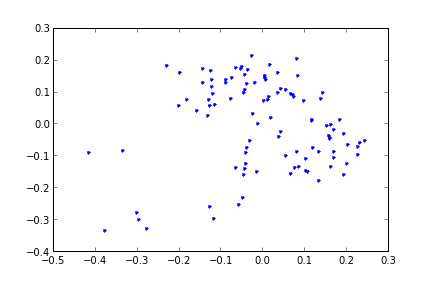
\includegraphics[height=6cm]{pca_4.png}

Simdi ayni veriyi bir de etiket bilgisini devreye sokarak
cizdirelim. Sanat kirmizi muzik mavi olacak.

\begin{minted}[fontsize=\footnotesize]{python}
arts =proj[labels == 'art']
music =proj[labels == 'music']
plt.plot(arts[:,0],arts[:,1],'r.')
plt.plot(music[:,0],music[:,1],'b.')
plt.savefig('pca_5.png')
\end{minted}

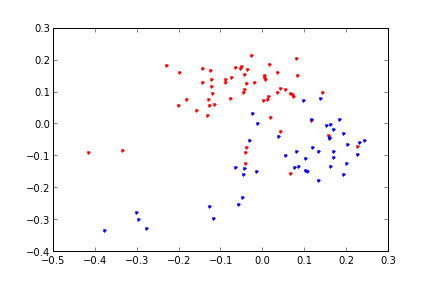
\includegraphics[height=6cm]{pca_5.png}

Goruldugu gibi veride ortaya cikan / ozvektorlerin kesfettigi dogal
ayirim, hakikaten dogruymus.

Metotun ne yaptigina dikkat, bir suru boyutu bir kenara atmamiza
ragmen geri kalan en onemli 2 boyut uzerinden net bir ayirim ortaya
cikartabiliyoruz. Bu PCA yonteminin iyi bir is becerdigini gosteriyor,
ve kelime sayilarinin makalelerin icerigi hakkinda ipucu icerdigini
ispatliyor.



Kaynaklar

[1] Alpaydin, E., Introduction to Machine Learning, 2nd Edition

[2] Strang, G., Linear Algebra and Its Applications, 4th Edition

[3] \url{http://www.stat.columbia.edu/~fwood/Teaching/w4315/Spring2010/PCA/slides.pdf}

[4] Cosma Rohilla Shalizi, Advanced Data Analysis from an Elementary
Point of View

[5] \url{http://www.ldc.upenn.edu/Catalog/CatalogEntry.jsp?catalogId=LDC2008T19}

[6] \url{http://www.stat.cmu.edu/~cshalizi/490/pca}

[7] \url{http://www.math.nyu.edu/faculty/goodman/teaching/RPME/notes/Section3.pdf}

[8] Lineer Cebir notlarimizda SVD turetilmesine bakinca ozdeger/vektor
mantigina atif yapildigini gorebiliriz ve akla su gelebilir; "ozdeger
/ vektor rutini isletmekten kurtulalim dedik, SVD yapiyoruz, ama onun
icinde de ozdeger/vektor hesabi var".  Fakat sunu belirtmek gerekir ki
SVD numerik hesabini yapmanin tek yontemi ozdeger/vektor yontemi
degildir. Mesela Numpy Linalg kutuphanesi icindeki SVD, LAPACK dgesdd
rutinini kullanir ve bu rutin ic kodlamasinda QR, ve bir tur bol /
istila et (divide and conquer) algoritmasi isletmektedir.






\end{document}
